%%% template.tex
%%%
%%% This LaTeX source document can be used as the basis for your technical
%%% paper or abstract. Regardless of the length of your document, the commands
%%% are all the same.
%%% 
%%% The "\documentclass" command is the first command in your file. If you want to 
%%% prepare a version of your article with line numbers - a "review" version - 
%%% include the "review" parameter:
%%%    \documentclass[review]{acmsiggraph}
%%%

\documentclass[review]{acmsiggraph}

%%% Title of your article or abstract.

\title{Depth Estimation in Scenes with Reflective Surfaces}

\author{Stephen N. Spencer\thanks{e-mail:spencer@cs.washington.edu}\\Chair, ACM SIGGRAPH Publications Committee}
\pdfauthor{Stephen N. Spencer}

%%% Used by the ``review'' variation; the online ID will be printed on 
%%% every page of the content.

\TOGonlineid{45678}

% User-generated keywords.
\keywords{time-of-flight, depth refinement, gated time-of-flight, shuttered light pulse}

% With the "\setcopyright" command the appropriate rights management text will be added
% to your document.

%\setcopyright{none}
%\setcopyright{acmcopyright}
%\setcopyright{acmlicensed}
\setcopyright{rightsretained}
%\setcopyright{usgov}
%\setcopyright{usgovmixed}
%\setcopyright{cagov}
%\setcopyright{cagovmixed}
%\setcopyright{rightsretained}

% The year of publication in the "\copyrightyear" command.

\copyrightyear{2016}

%%% Conference information, from the completed rights management form.
%%% The "\conferenceinfo" command has two parameters: 
%%%    - conference name
%%%    - conference date and location
%%% The "\isbn" field includes the year and month after the article ISBN.

\conferenceinfo{SIGGRAPH 2016 Posters}{July 24-28, 2016, Anaheim, CA} 
\isbn{978-1-4503-ABCD-E/16/07} 
\doi{http://doi.acm.org/10.1145/9999997.9999999}

% Load basic packages
\usepackage{graphics} % for EPS, load graphicx instead
\usepackage{url}      % llt: nicely formatted URLs
\usepackage{float}
\usepackage{array}
\usepackage{amsfonts} % For mathbb
\usepackage{amstext} % for \text in math mode
\usepackage{amsmath} % for math
\usepackage{amssymb}
\usepackage{amsmath}
\usepackage{mathtools}
\usepackage{graphicx}
\usepackage{caption}
% \usepackage{subcaption}
\usepackage{subfigure}
\usepackage{fancyvrb}
\usepackage{color}
\usepackage{algpseudocode}
\usepackage{bbm}
\usepackage[dvipsnames]{xcolor}
\DeclarePairedDelimiter\norm{\lVert}{\rVert}%
% \usepackage{ruler}

\DeclareMathOperator*{\argmin}{argmin}

% Author comments
\newcommand{\srinath}[1]{\textcolor{red}{[\textbf{Srinath}]: #1}} % Srinath
\newcommand{\shahram}[1]{\textcolor{green}{[\textbf{Shahram}]: #1}}
\newcommand{\CHT}[1]{\textcolor{blue}{[\textbf{CT}: #1]}}
\newcommand{\Dan}[1]{\textcolor{YellowOrange}{[\textbf{Dan}: #1]}}

% Custom defines
% \newcommand{\ie}{\emph{i.e.\ }}
% \newcommand{\eg}{\emph{e.g.\ }}
% \newcommand{\etal}{\emph{et al.\ }}
\newcommand{\parahead}[1]{\setlength{\parindent}{0cm}\par\textbf{#1}:\ }
\newcommand{\tabhead}[1]{\par\textbf{#1}}
% Packed itemize
\newenvironment{packed_itemize}
{\begin{itemize}
    \setlength{\itemsep}{1pt}
    \setlength{\parskip}{0pt}
    \setlength{\parsep}{0pt}
}{\end{itemize}}

\newcommand{\R}{\mathbb{R}}
\newcommand{\vect}[1]{\mathbf{#1}}
\newcommand{\B}{\mathcal{B}}
\newcommand{\K}{\mathcal{K}}
\newcommand{\E}{E}

\newcommand{\MU}{\boldsymbol{\mu}}
\newcommand{\C}{\mathcal{C}}
\newcommand{\G}{\mathcal{G}}

\newcommand{\filluptopage}[1]{%
  \clearpage
  \loop\ifnum\value{page}<#1\relax
    \null\clearpage
  \repeat
  \loop\ifnum\value{page}=#1\relax
    \null\clearpage
  \repeat
}

\begin{document}

%%% This is the ``teaser'' command, which puts an figure, centered, below 
%%% the title and author information, and above the body of the content.

\teaser{
  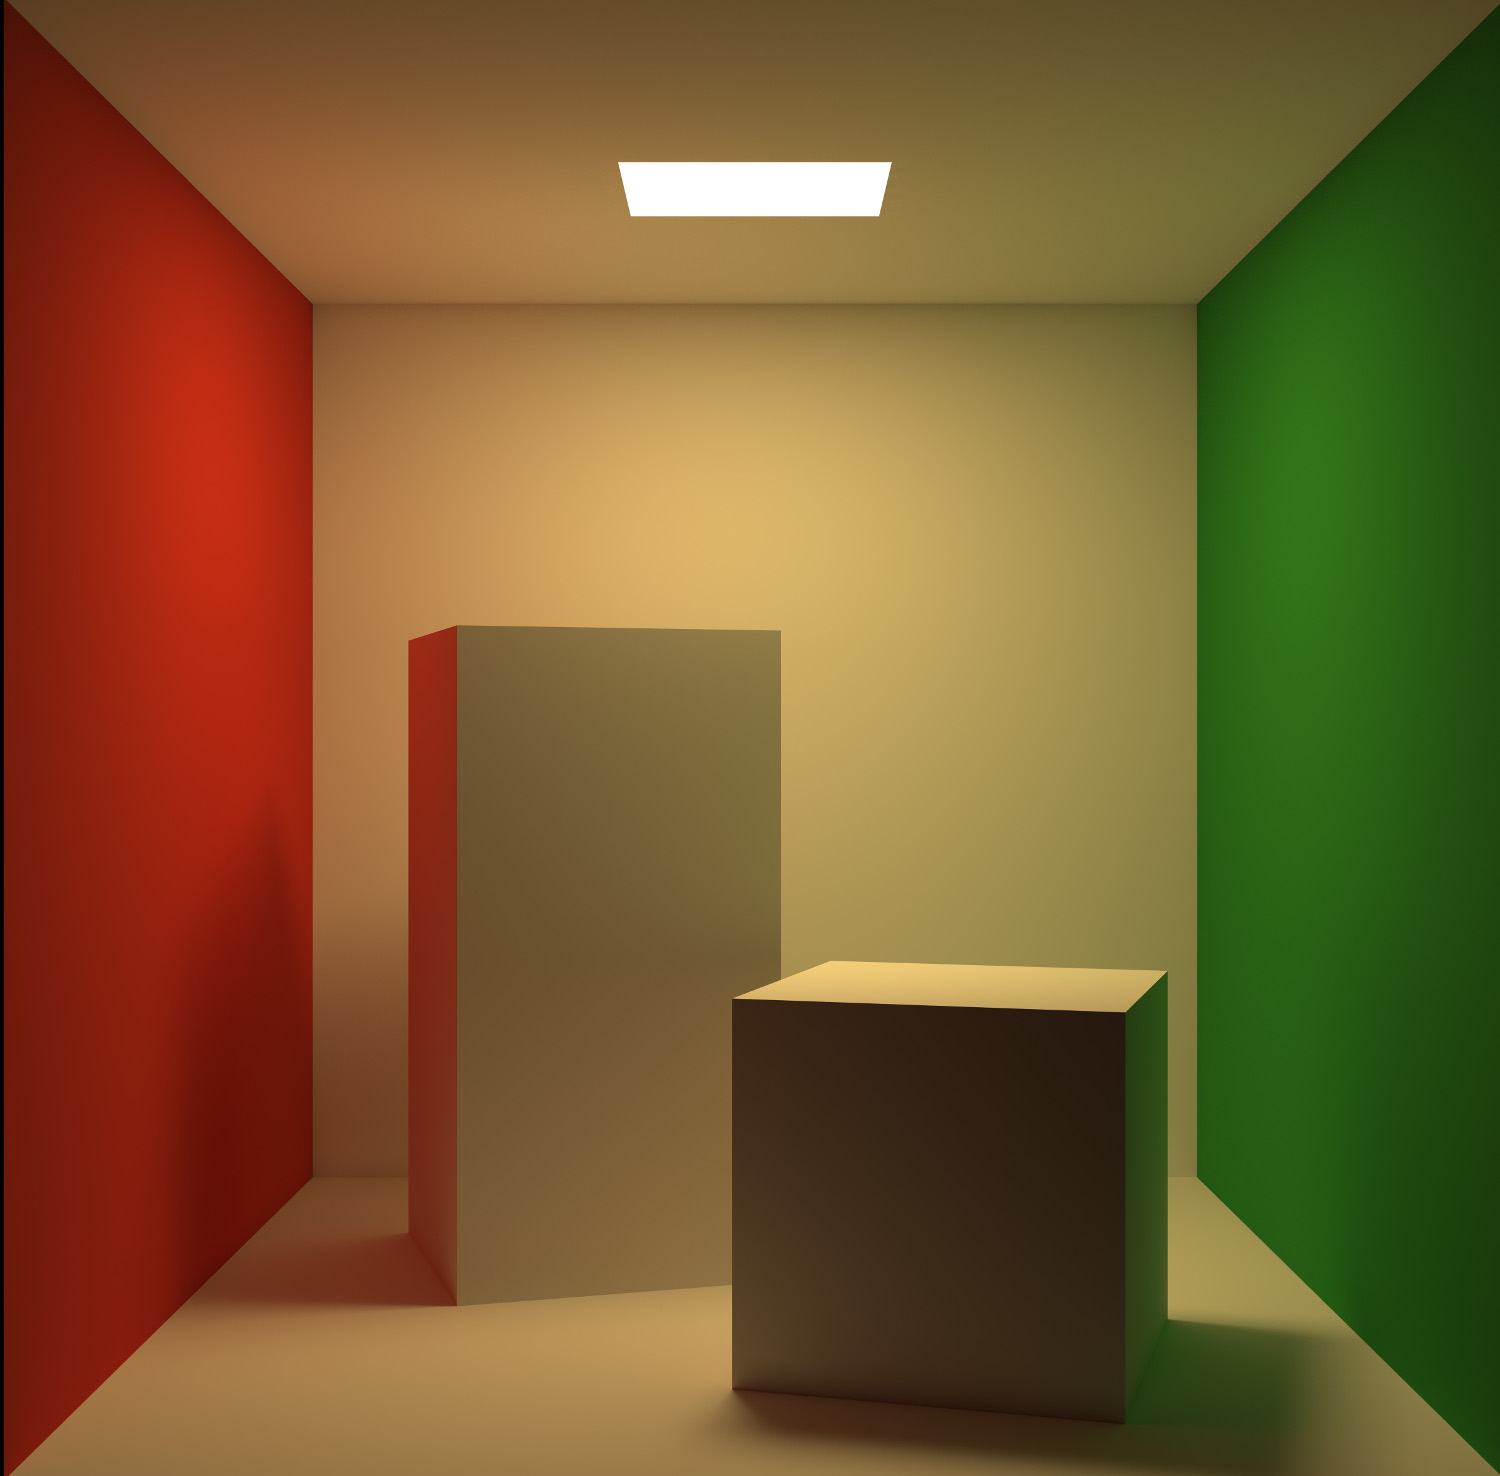
\includegraphics[height=1.5in]{content/images/teaser.jpg}
  \caption{Nice teaser showing gist of technique or cool results goes here.}
 }

\maketitle

\begin{abstract}

\end{abstract}
\section{Introduction}
% \srinath{TODO: General introdcution with motivation and summary of state of the art.}

\subsection{Goal}
We are imaging a scene containing objects of unknown geometry and known to contain a specular reflector within the field of view.
Our goal is to estimate a 3D point set $P$ lying on the surface of objects of interest in the scene.
To this end, we use information from direct and indirect (\emph{e.g.} reflections, multipath due to reflection) image observations.
The input to our method consists of shutter images $S_t$ at each time instant from CW or gated time-of-flight sensors, and known pose of the camera and the reflector.

\subsection{Assumptions}
In the first iteration of this method, we make the following assumptions.
\begin{itemize}
\item The pose of the reflector relative to the camera is known.
\item The reflector is a flat, perfect mirror.
\item Multipath effects other than those due to the mirror are ignored.
\item Known template mesh of the model? (if we end up using an iterative solution to estimate normals)
\end{itemize}

\subsection{Geometric Solution to Enriching Depth Estimates}
There are 5 different types of pixels that will be observed in shutter images $S_t$ when the imaging a scene contains a reflector, see Figure~\ref{fig:types_of_pixels}.

\subsection{Hand Tracking with Estimated Point Set}

\subsection{Relaxations and Future Extensions}
\begin{itemize}
\item Estimate confidence of each pixel since we have mulitple reflections.
\item Relax Assumptions: Both camera and reflector move.
\item Relax Assumptions: Imperfect reflector.
\item Relax Assumptions: Non-flat reflector.
\item Reconstruction of surface reflectance properties.
\end{itemize}

\subsection{Random Points for Paper}
\begin{itemize}
  % 
\item Reviewers may ask: Why note use a structured light sensor? In a structured light sensor, the parts that are seen twice (i.e. the mulitpath pixels in ToF) also are covered by the structured light pattern twice. Resolving this is as hard/harder as resolving multipath. \Dan{I've seen multiple structure light setups working together i.e: \url{https://www.cs.unc.edu/~maimone/media/kinect_VR_2012.pdf}}
  % 
\item Can make a figure: along x-axis we have line of sight imaging, partial LOS+out of sight, fully out of sight. What should be along Y-axis?. The reason why ours is a hard problem is because we do partial LOS+out of sight using a mirror. Much harder due to multipath.
  % 
\item For evaluation, we would need to show why we need this depth correction. What would happen if we do tracking on the uncorrected (but ray folded) depths? My guess is the noise would kill the tracking. Then we need to show that the correction improves things quite a bit and helps because we now have all this extra information.
  % 
\end{itemize}

Applications that would appeal to a SIGGRAPH audience. These random scribbles need to be 
\begin{itemize}
\item Games in which people play in front of mirror with their own reflection of hands and maybe full body.
\item Tracking the mirror is cool. This means we can augment the mirror with content.
\item Summary title: Using multipath for fun and profit
\item Use a mirror as a display since you can render stuff on the mirror
\end{itemize}

More miscellaneous ideas.

\begin{itemize}
\item Apply bilateral filter to raw ir
\item Do background subtraction before tracking hands in the reflection. This gives super clear results
\item Order two way mirror sample for testing
\item Interactive AR editing on a whiteboard (could just be one of many possible applications). Person writes something on a reflective whiteboard. This text/image can be recognized/animated, perhaps in 3D together with hand tracking.\item Tablet/monitor/phone/display replacement with hand-based interaction
\item Tabletop interaction
\item In the future, it's not unreasonable to assume that walls will be painted with IT retroreflectors and lights will be modulated IR lights. This information can be leveraged for ToF
\item It's ok to make certain hardware assumptions (painted surfaces, fixed cameras)
\item Light field imaging can be done :)
\end{itemize}
\section{Model of Multipath due to Highly Reflective Material}
In this section we describe the formulation that we use to model the incident light at each pixel of the image.
We assume that the imaged scene contains a direct view of the object of interest as well as a reflection of it.
This causes multipath interference--our goal is to estimate true depths in the presense of multipath.

Consider the usual measurement from a camera in the absense of any multipath effects.
Without loss of generality, we assume that the object of interest is Lambertian.
This is a reasonable assumption to make~\cite{somepaper}, but our model could further be extended to non-Lambertian materials if necessary.
%
\begin{figure}
\centering
  %
  \subfigure[Single bounce]
  {
    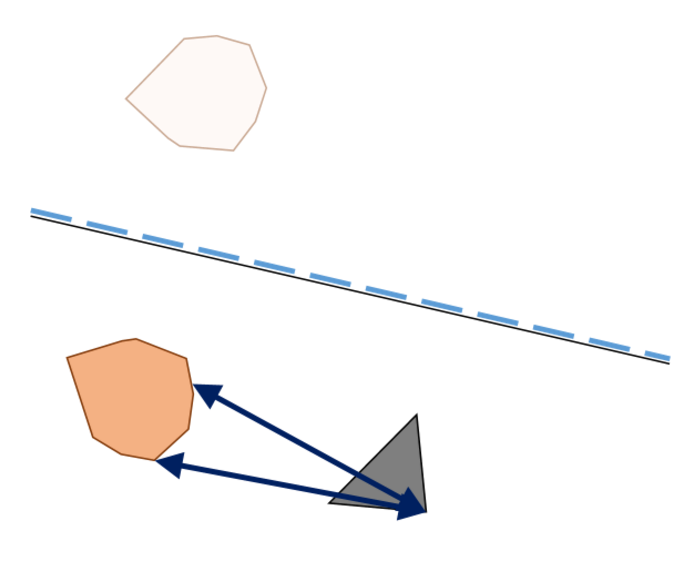
\includegraphics[width=0.19\textwidth]{content/images/1_bounce.png}
    \label{fig:single_bounce}
  }
  % 
  \subfigure[Three bounce]
  {
    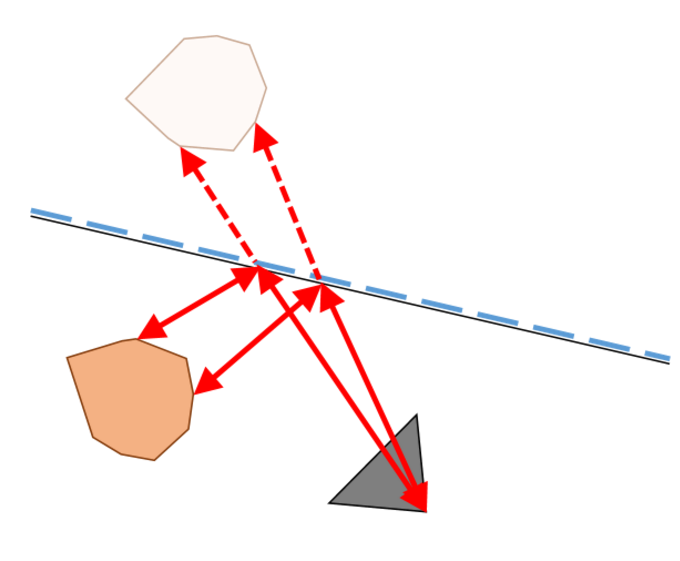
\includegraphics[width=0.19\textwidth]{content/images/3_bounce.png}
    \label{fig:three_bounce}
  }
  % 
  \subfigure[\textbf{Multipath}: 1 + 2 bounce]
  {
    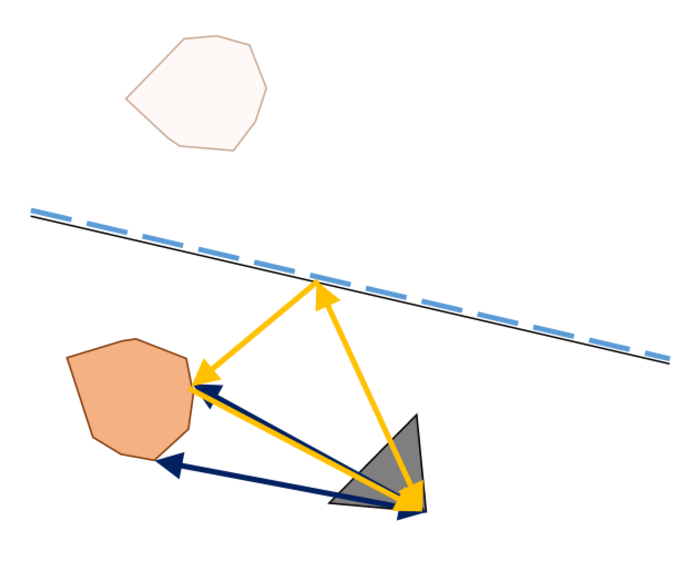
\includegraphics[width=0.19\textwidth]{content/images/21_bounce.png}
    \label{fig:1_2_bounce}
  }
  % 
  \subfigure[\textbf{Multipath}: 3 + 2 bounce]
  {
    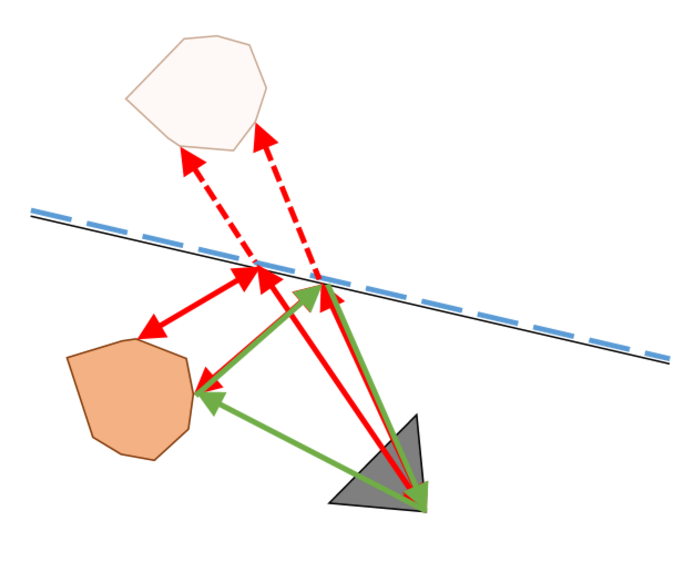
\includegraphics[width=0.19\textwidth]{content/images/32_bounce.png}
    \label{fig:3_2_bounce}
  }
  % 
  \subfigure[Single bounce from mirror]
  {
    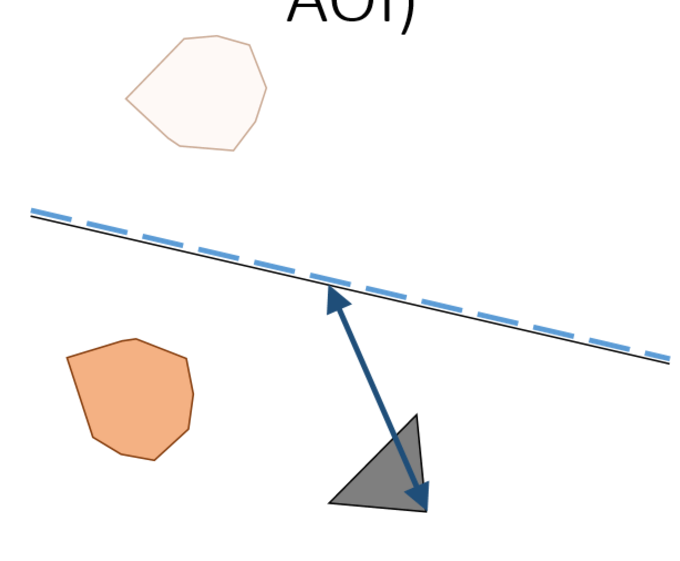
\includegraphics[width=0.19\textwidth]{content/images/1_bounce_mirror.png}
    \label{fig:single_bounce_mirror}
  }
  \caption{Types of pixels}
  \label{fig:types_of_pixels} 
\end{figure}

The radiant intensity at each pixel in the image is given by
%
\begin{align}
r = \frac{m_o \, I}{d^2} \, \max{(\mathbf{L} \cdot \mathbf{n}, 0)},
\end{align}
%
where, $m_o$ is the albedo of the object,
$\mathbf{L}$ is the normalized incident light direction,
$\mathbf{n}$ is the surface normal,
$I$ is the intensity of the light source, and
$d$ is the radial distance from the camera to the surface point.

For a (gated) TOF sensor, the light intensity is further modulated.
Let $C_i(d)$ denote the modulation factor at different phase shifts (also called the \emph{calibration curve}).
Contatenating multiple phase or frequency measurements from the TOF sensor at each pixel, we have,
%
\begin{align}
\mathbf{R} = m_o \, I \, \max{(\mathbf{L} \cdot \mathbf{n}, 0)} \, \mathbf{C}(d).
\end{align}
%
Note that the attenuation of light due to distance from the light source is modeled by $\mathbf{C}(d)$.

\begin{figure}
\centering
		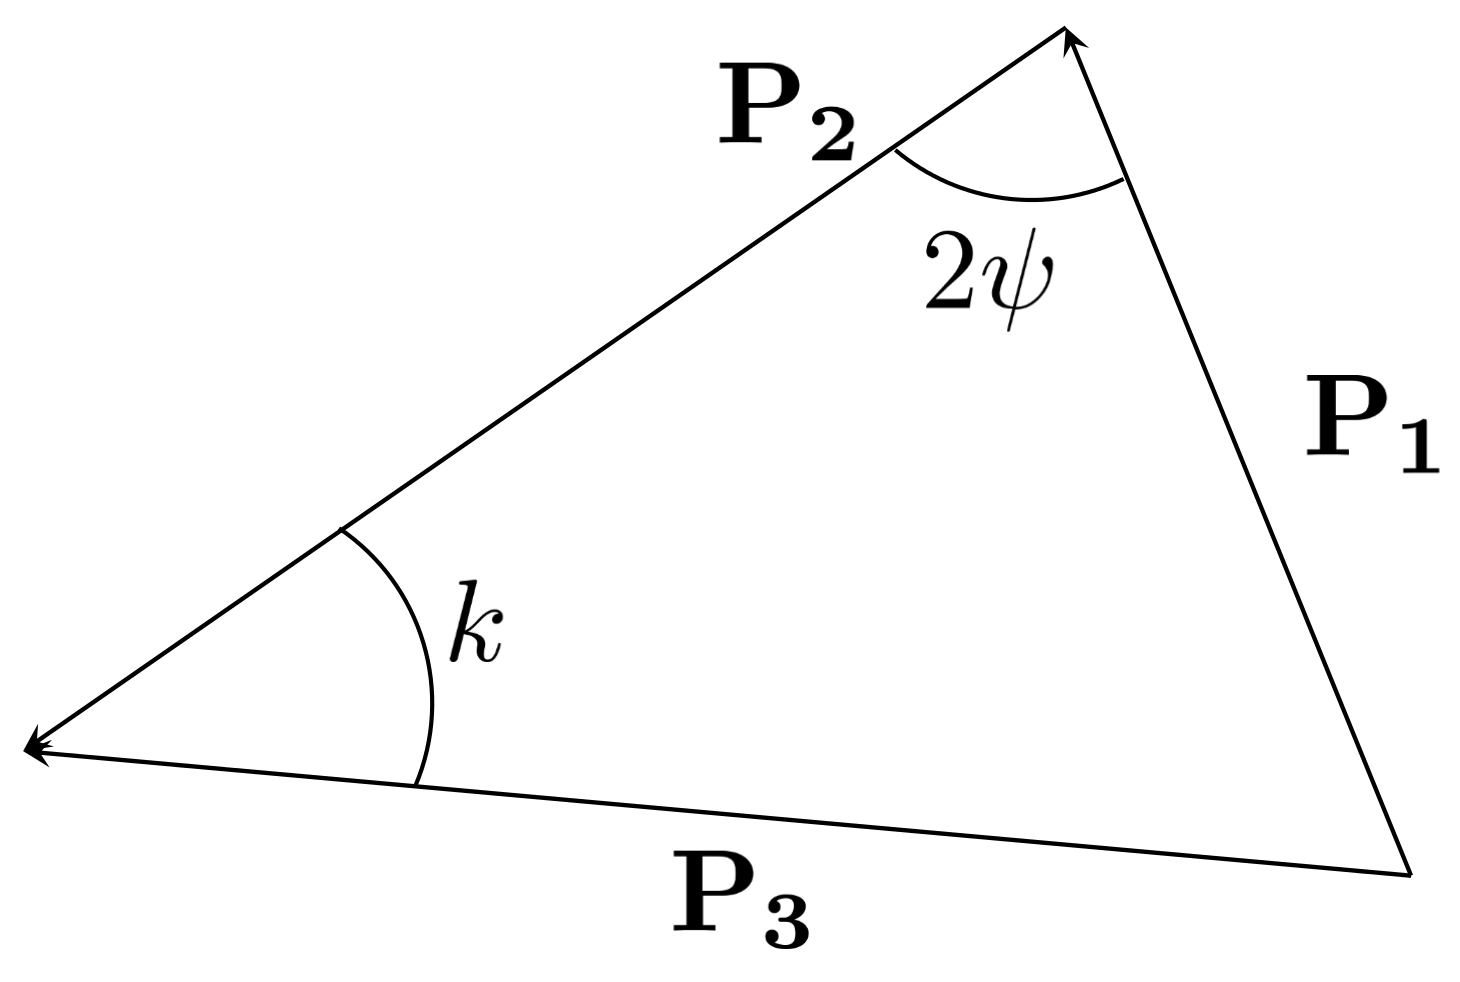
\includegraphics[width=0.8\columnwidth]{content/images/MultipathTriangle/MultipathTriangle.png}
		\caption{The multipath triangle.}
		\label{fig:multipath_triangle}
\end{figure}


\subsection{Reflectance Model for Highly Reflective Surfaces}
We now consider the case when a TOF sensor views a part of the scene that is measured directly but also contains reflection from the mirror (see Figure~\ref{fig:1_2_bounce}). We call this case \textbf{Bounce12} to mean that the first bounce interferes with the second bounce. The radiant intensity at each such pixel is given by
%
\begin{align}
\mathbf{R_{12}} = m_o \, I \, \max{(\mathbf{L_d} \cdot \mathbf{n}, 0)} \, \mathbf{C}(d_1)\nonumber \\
					 + \, m_o \, m_m \, I \, \max{(\mathbf{L_r} \cdot \mathbf{n}, 0)} \, \mathbf{C}(d_2),
\end{align}
%
where, $\mathbf{L_d}$ is the direction of light from the camera to the surface directly,
$\mathbf{L_r}$ is the direction of light from the camera to the surface \emph{after} reflection on the mirror, $d_1$ and $d_2$ are the radial distances along the direct and reflected paths respectively from light source back to the sensor, and $m_m$ is the albedo of a mirror which is usually $1.0$.
%
In terms of the \emph{multipath triangle} (Figure~\ref{fig:multipath_triangle}), $d_1 = P_3$ and $d_2 = (P_1 + P_2 + P_3) / 2.$
Substituting for $m_m$, we can write the above equation upto a scaling factor as,
%
\begin{align}
\mathbf{R_{12}} \propto \max{(\mathbf{L_d} \cdot \mathbf{n}, 0)} \, \mathbf{C}(d_1) 
					 + \max{(\mathbf{L_r} \cdot \mathbf{n}, 0)} \, \mathbf{C}(d_2).
\end{align}
%

Following a similar reasoning, we can write the radiant intensity at each pixel for the second multipath case, \textbf{Bounce32}, as
%
\begin{align}
\mathbf{R_{32}} = m_o \, m_m \, I \, \max{(\mathbf{L_r} \cdot \mathbf{n}, 0)} \, \mathbf{C}(d_3)\nonumber \\
					 + \, m_o \, I \, \max{(\mathbf{L_d} \cdot \mathbf{n}, 0)} \, \mathbf{C}(d_2),
\end{align}
%
which simplifies to
%
\begin{align}
\mathbf{R_{32}} \propto \max{(\mathbf{L_r} \cdot \mathbf{n}, 0)} \, \mathbf{C}(d_3)
					 + \max{(\mathbf{L_d} \cdot \mathbf{n}, 0)} \, \mathbf{C}(d_2).
\end{align}
%
In terms of the \emph{multipath triangle} (Figure~\ref{fig:multipath_triangle}), $d_2 = (P_1 + P_2 + P_3) / 2$ and $d_3 = P_1 + P_2.$
%
%\Dan{To me looks like $d_2 = (P_1 + P_2 + P_1) / 2$ }
Finally, we can write the radiant intensity at each pixel for the two multipath cases after substitution as follows.
%
\begin{align}
\mathbf{R_{12}} \propto & \max{(\mathbf{L_d} \cdot \mathbf{n}, 0)} \, \mathbf{C}(P_3) \nonumber\\
					 & + \max{(\mathbf{L_r} \cdot \mathbf{n}, 0)} \, \mathbf{C}\left(\frac{P_1 + P_2 + P_3}{2}\right),
		\label{eqn:R12}
\end{align}
%
and
\begin{align}
%
\mathbf{R_{32}} \propto & \max{(\mathbf{L_r} \cdot \mathbf{n}, 0)} \, \mathbf{C}(P_1 + P_2)\nonumber\\
					& + \max{(\mathbf{L_d} \cdot \mathbf{n}, 0)} \, \mathbf{C}\left(\frac{P_1 + P_2 + P_3}{2}\right).
		\label{eqn:R32}
\end{align}
%

\subsection{Factoring Surface Normals Out}
In the above equations for multipath, the surface normal $\mathbf{n}$ is often not available beforehand.
In order to still be able to estimate the calibration curves, we would like to factor the normal out.

\begin{figure}
\centering
		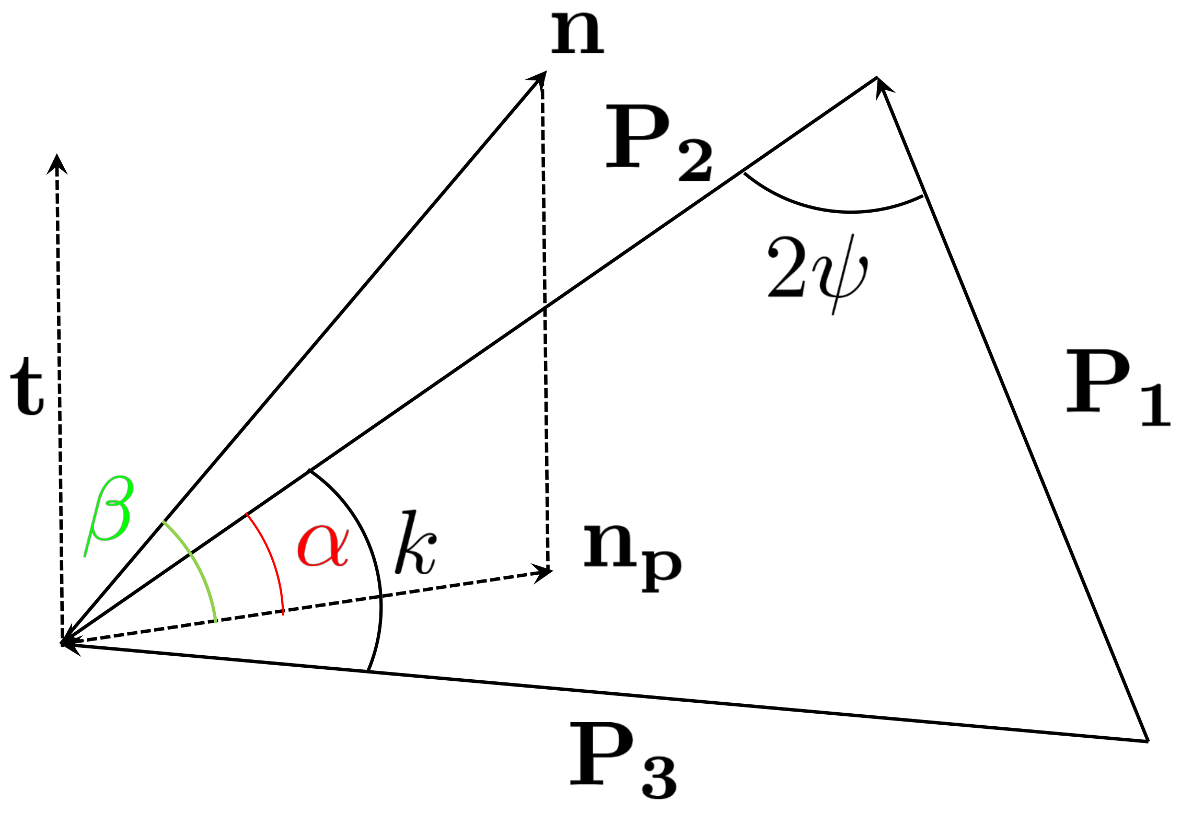
\includegraphics[width=0.8\columnwidth]{content/images/MultipathTriangle/MultipathTriangle_Normal.png}
		\caption{Projecting surface normal on multipath triangle. Here $\mathbf{n}$ is the surface normal and $\mathbf{n_p}$ is its projection on the plane containing the multipath triangle. $\alpha$ is the angle between $\mathbf{n_p}$ and $\mathbf{P_2}$, and $\beta$ is the angle between $\mathbf{n_p}$ and $\mathbf{n}$.}
		\label{fig:multipath_normals}
\end{figure}

Figure~\ref{fig:multipath_normals} shows how the effect of the normal can be factored out by projecting it on the plane containing the multipath triangle.
Let $\mathbf{n_p}$ be the projection of the normal on the multipath triangle.
This is given by,
%
\begin{align}
%
\mathbf{n_p} & = \mathbf{n} - \left(\mathbf{n} \cdot \mathbf{t}\right) \mathbf{t}\nonumber\\
& = \mathbf{n} - \cos(90 - \beta) \, \mathbf{t}\nonumber\\
& \left[\text{Since $\mathbf{n}$ and $\mathbf{t}$ are unit vectors.}\right]\nonumber
%
\end{align}
%
where $\mathbf{t}$ is the normal to the plane containing the multipath triangle, and $\beta$ is as shown in the figure.
Thus, we can write the surface normal to be,
%
\begin{align}
\mathbf{n} & = \mathbf{n_p} + \sin(\beta) \, \mathbf{t}.
\label{eqn:normal_projection}
\end{align}
%
Note that while $\mathbf{n}$ and $\mathbf{t}$ are unit vectors, $\mathbf{n_p}$ is not.
We can now substitute Equation~\ref{eqn:normal_projection} in Equations~\ref{eqn:R12} and ~\ref{eqn:R32} .
Along with the observation that $\mathbf{L_r} \cdot \mathbf{t} = 0$ and $\mathbf{L_d} \cdot \mathbf{t} = 0$,
we can write the dot products as,
%
\begin{align}
\mathbf{L_d} \cdot \mathbf{n} = \mathbf{L_d} \cdot \mathbf{n_p} &= ||\mathbf{n_p}|| \,
\cos(k - \alpha),\nonumber\\
\mathbf{L_r} \cdot \mathbf{n} = \mathbf{L_r} \cdot \mathbf{n_p} &= ||\mathbf{n_p}|| \, \cos{\alpha}\nonumber.
\end{align}
%
\Dan{This needs some check, $\mathbf{L_d} \cdot \mathbf{n} = \mathbf{L_d} \cdot \mathbf{n_p}$ is not true?}

where $k$ is the angle between $L_r$ and $L_d$.
Note that $\mathbf{L_d} = \frac{\mathbf{P_3}}{||\mathbf{P_3}||}$, and
$\mathbf{L_r} = \frac{\mathbf{P_2}}{||\mathbf{P_2}||}$.

Using the fact that the norm of a vector is always positive, and that $||\mathbf{n_p}||$ is common in both the above equations,
we can rewrite Equations~\ref{eqn:R12} and \ref{eqn:R32} as,
%
\begin{align}
\mathbf{R_{12}} \propto & \max{(\cos(k - \alpha), 0)} \, \mathbf{C}(P_3) \nonumber\\
					 & + \max{(\cos(\alpha), 0)} \, \mathbf{C}\left(\frac{P_1 + P_2 + P_3}{2}\right),
\end{align}
%
and
\begin{align}
\mathbf{R_{32}} \propto & \max{(\cos(\alpha), 0)} \, \mathbf{C}(P_1 + P_2)\nonumber\\
					& + \max{(\cos(k - \alpha), 0)} \, \mathbf{C}\left(\frac{P_1 + P_2 + P_3}{2}\right),
\end{align}
where $-90 < \alpha < 90$.
By convention, $\alpha$ is positive when it is in the direction of $\mathbf{P_2}$ to $\mathbf{P_3}$ and negative in the other direction.
We do not consider $|\alpha| \ge 90$ since the intensity falls to zero for a Lambertian reflectance model under such conditions.


\bibliographystyle{acmsiggraph}
\nocite{*}
\bibliography{content/HandTOF}
\end{document}

\end{document}
